\section{Classical results}
\label{sec:classical-results}

Results below are production ensembles at $N=3000$ quarks (48 events per
expansion-rate point; the multiquark-favorable ``corner'' uses
$\alpha_s=0.6$, $H_0=0.05\,c/\fm$, and twelve injected $c\bar c$ pairs,
24 events), validated across a seventeen-fold volume range: per-quark
meson-bound fractions are $13.1\%$, $12.9\%$, $13.0\%$ at $N=604$,
$3000$, $10^4$, with composite rates scaling within $1\sigma$
(Appendix~\ref{app:validation}, which also collects the full
systematics table).

\begin{figure*}[t]
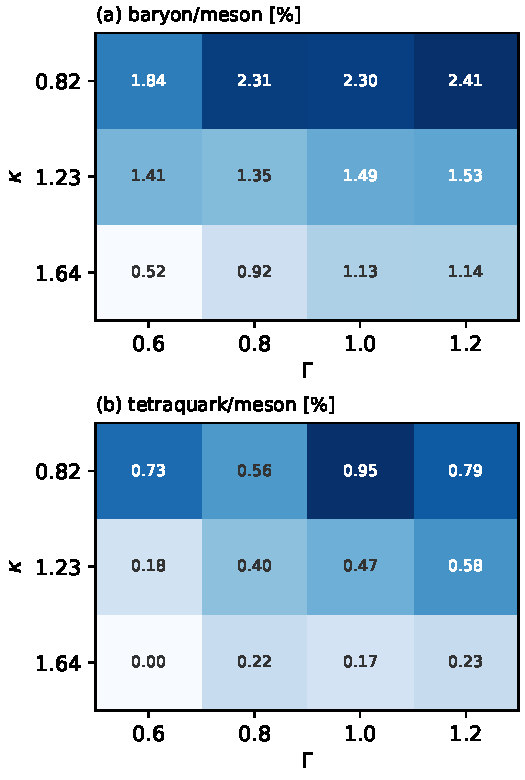
\includegraphics[width=0.85\textwidth]{figs/fig11_heatmap.pdf}
\caption{Composite-to-meson ratios across the coupling--screening
plane ($N=3000$, 16 events per cell).  Both ratios grow monotonically
with $\Gamma$ and with decreasing $\kappa$ (longer-ranged
attraction); $B/M$ spans $0.5$--$2.4\%$ and $T/M$ reaches $\sim1\%$
at the strongest-coupling, weakest-screening corner.  The
diquark-first fraction is $0.81$--$0.95$ over the entire plane.}
\label{fig:heatmap}
\end{figure*}

Figure~\ref{fig:heatmap} maps the composite-to-meson ratios over the
full coupling--screening plane: both rise monotonically toward strong
coupling and weak screening, with $B/M$ sweeping $0.5$--$2.4\%$
(bracketing the direction of the measured $p/\pi^+\approx5\%$) and
$T/M$ reaching the percent level --- while the diquark-first fraction
never leaves the $0.81$--$0.95$ band, making the amplification of the
static estimate a plane-wide, not point-specific, conclusion.

\subsection{Static limit}

The static machinery of Ref.~\cite{Lebed:2016jvq} is reproduced
exactly --- our closed-form estimator [Eq.~\eqref{eq:pstatic}] matches
every hard-wall entry of his Tables~1--2 to all quoted digits, and the
ideal-gas Monte Carlo agrees in both counting modes
(Appendix~\ref{app:color}, where the $\sim9$-point difference between
his channel counting and the discrete-color counting is quantified as
the prescription systematic).  One static result is new: applying the
estimator to \emph{interacting} equilibrated configurations at the
simulation's density ($n_0R^3=1$, $\Gamma\approx0.8$, 64 paired seeds
at $N=3000$) shifts the probability by
$-0.0004\pm0.0035$ (Lebed counting) and $+0.0009\pm0.0033$ (discrete)
--- zero.  The nearest-neighbor estimate is robust not only to
screening assumptions, as Ref.~\cite{Lebed:2016jvq} showed, but to
liquid-state correlations; the interesting physics is therefore
entirely in the dynamics.

\subsection{Species formation in the expanding plasma}

\begin{figure}[t]
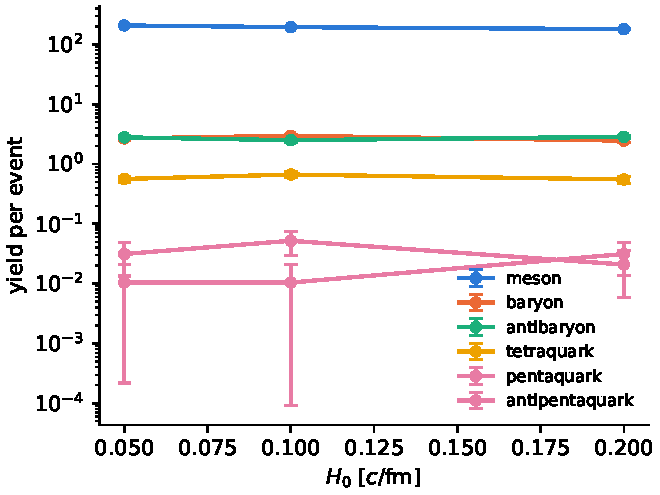
\includegraphics[width=\columnwidth]{figs/fig5_scan_H0.pdf}
\caption{Species yields per event versus expansion rate $H_0$
($N=3000$, 48 events/point, bootstrap errors).  Faster quenches capture
fewer mesons; the tetraquark yield is flat within errors across the
factor-of-four range of quench rates.}
\label{fig:scanH0}
\end{figure}

\begin{figure}[t]
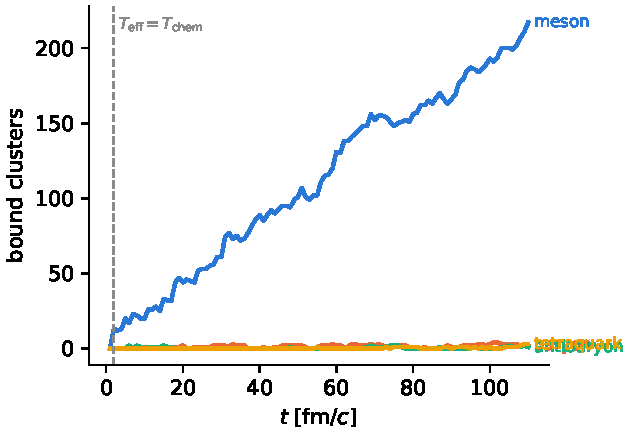
\includegraphics[width=0.9\columnwidth]{figs/fig4_species_t.pdf}
\caption{Bound-cluster counts per snapshot for one event at default
parameters ($N=3000$, $H_0=0.1\,c/\fm$; the dashed line marks the
$\Tchem$ crossing).  Mesons condense gradually as the Hubble redshift
drains relative kinetic energy; (anti)baryons and transient
tetraquarks appear late.}
\label{fig:speciest}
\end{figure}

Across $H_0 = 0.05$--$0.20\,c/\fm$ the meson yield falls from
$207.4\pm1.7$ to $181.9\pm1.5$ per event, (anti)baryons sit at
$2.3$--$2.9$ per species, and --- notably --- the tetraquark yield is
\emph{flat} at $0.58\pm0.10$ per event across the full factor of four
in quench rate (Fig.~\ref{fig:scanH0}).  Five-quark states appear at
every expansion rate once both charge states are counted: with 96
seeds at the two slower points, $4$ and $6$ (anti)pentaquarks
($0.042$ and $0.062$ per event), and $3$ in 48 events at
$H_0=0.2\,c/\fm$, with no significant $H_0$ trend.  A
single-event history is shown in Fig.~\ref{fig:speciest}, and
Fig.~\ref{fig:render} renders the assembly process: particles colored
by their \emph{eventual} species are uncorrelated at early times,
partially clustered at mid-evolution, and tightly paired at
freeze-out.

\begin{figure*}[t]
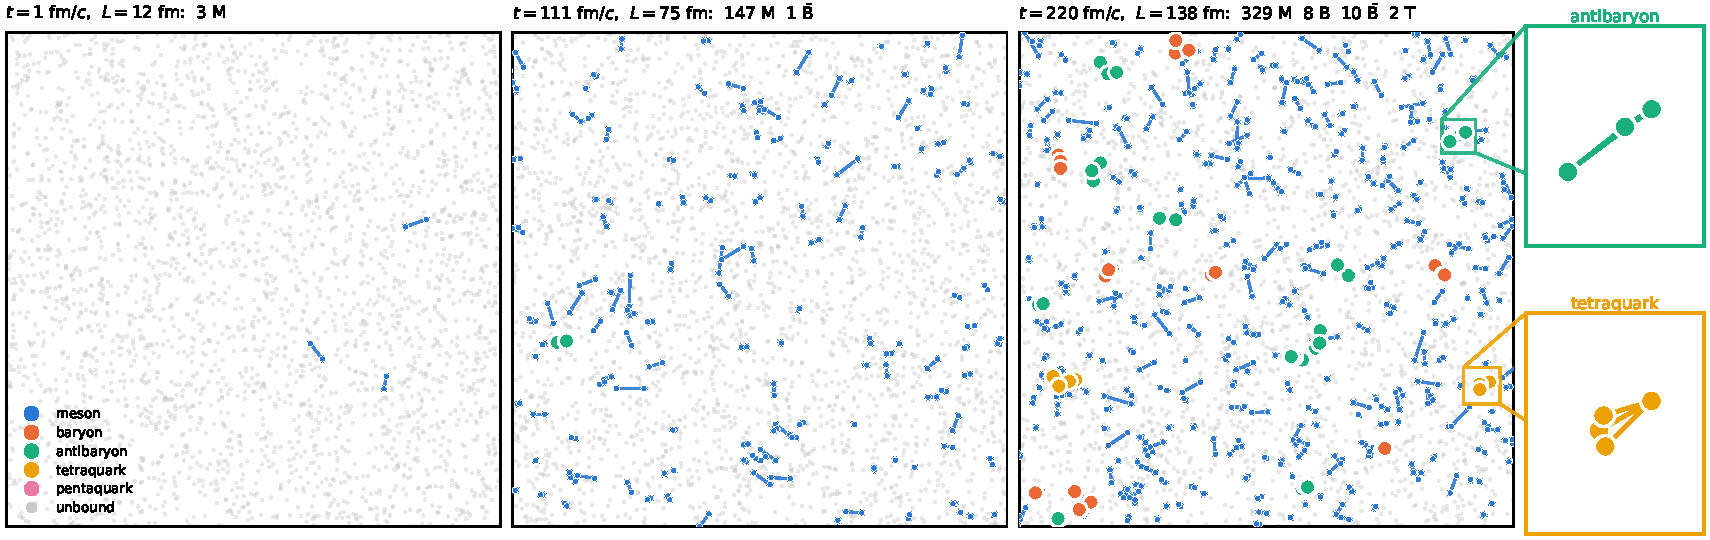
\includegraphics[width=\textwidth]{figs/fig3_render.pdf}
\caption{One event at the most productive point of the
coupling--screening plane ($\alpha_s=0.6$, $\lambda_{D,0}=0.6\fm$,
i.e.\ $\Gamma\approx1.2$, $\kappa\approx0.82$; $H_0=0.05\,c/\fm$,
$N=3024$) at three times, full-box projection.  Members of eventual
clusters are colored and bonded once the cluster has assembled (all
pair separations within $1.2\,\lambda_D(t)$); everything else is gray.
The plasma at $t=1\fm/c$ carries almost no assembled structure; mesons
condense as bonded pairs through mid-evolution; the final panel holds
$329$ mesons, $18$ (anti)baryons, and two tetraquarks, with insets
zooming a three-quark baryon and a four-body tetraquark.}
\label{fig:render}
\end{figure*}

\subsection{Constituent-number penalty}

\begin{figure}[t]
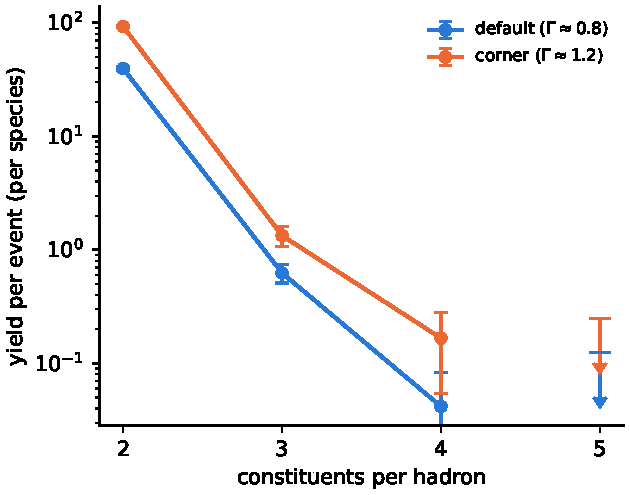
\includegraphics[width=\columnwidth]{figs/fig6_penalty.pdf}
\caption{Yield per event (per species; particle and antiparticle states
averaged) versus constituent number at two couplings, $N=3000$.  All
four points are now measurements at both couplings.  The ladder is
$69\times$ ($2\to3$), $4.9\times$ ($3\to4$), and $19\times$ ($4\to5$)
at $\Gamma\approx0.8$, and $61\times$, $4.8\times$, $26\times$ at the
charm-enriched $\Gamma\approx1.2$ corner.}
\label{fig:penalty}
\end{figure}

The production ensembles resolve the full ladder
(Fig.~\ref{fig:penalty}): the meson$\to$baryon step costs
$\sim65\times$, but the ladder is \emph{not} geometric beyond it ---
adding a fourth constituent to a baryon-mass cluster costs only
$\sim5\times$, while the fifth costs $\sim20\times$.  The cheap $3\to4$
step reflects the combinatorics of the discrete-color model: a
tetraquark can be assembled from two already-attractive $q\bar q$ or
$qq$ sub-systems, whereas the first baryon requires three mutually
attractive quarks.  This deviation from the naive
constant-penalty-per-constituent expectation of coalescence
\cite{Fries:2008hs,ExHIC:2010gcb} is a concrete, testable output.

The strong-coupling corner delivered manifest flavor exotics: in 24
events, \emph{seven} tetraquarks and one antipentaquark whose net
flavor cannot be carried by any $q\bar q$ or $qqq$ assignment --- the
classical realization of the Tier-1 charge-exotic classification of
Sec.~\ref{sec:tier1} --- for an exotic-tetraquark yield of
$0.29\pm0.11$ per event.  Flavor-tagged re-runs of the exotic-bearing
events (bit-reproducible from archived seeds) show all eight are
\emph{light-flavor} exotics of the $dd\bar u\bar u$ / $ss\bar u\bar u$
class, and strangeness-rich: six of the eight carry strange quarks
beyond minimal content, the classical signature of mass-hierarchy
coalescence (slower $s$ quarks at fixed $T$ are captured more easily).
The $\Tcc$ analog itself did not occur: despite twelve $c\bar c$ pairs
per event, no $cc\bar q\bar q$ cluster formed
($<0.125$/event at 95\%~CL).  Biased seeding sharpens the diagnosis:
planting six \emph{pre-formed, bound} $cc$ diquarks per event at $t=0$
(144 seeded diquarks over 24 events) still produced zero charm
exotics --- the $\sim36\MeV$ diquark binding is no match for the
$T_0=200\MeV$ plasma, and the seeds melt in the first fm/$c$, each
charm quark ending in an ordinary charm meson.  Nor does planting at
the chemical freeze-out crossing help: a further 144 diquarks seeded
when $\Teff$ first falls below $\Tchem=160\MeV$ likewise produced
zero charm exotics --- chemical freeze-out is still four times hotter
than the diquark binding.  The classical model thus predicts
double-charm exotics to be \emph{doubly} suppressed: melted while the
medium is hot, partner-starved once it is dilute.  The seeded
diquark's melting curve completes the measurement: planting 144 bound
$cc$ diquarks per temperature at $\Teff = 160$, $80$, $40$, and
$20\MeV$ yields $0$, $0$, $0$, and $1$ charm exotics --- survival
turns on only \emph{below} the $\sim36\MeV$ binding energy, exactly
as melting arguments demand, and even then dressing succeeds at only
$\sim0.7\%$ per seed (the medium at $\Teff=20\MeV$ has expanded
sixteen-fold).  The lone survivor is a bona fide $\Tcc$ analog:
$cc\bar u\bar u$, net charm $+2$.  (The mid-run relocation perturbs
the light sector --- stranded partners of broken charm mesons inflate
the light-exotic count at late planting --- an artifact of the
surgical intervention that does not affect the charm-cluster count
itself.)

Exotic yields carry one dominant modeling uncertainty: under the
\texttt{max\_channel} color prescription (Appendix~\ref{app:color})
tetraquark and five-quark yields rise by factors of $12$ and $\sim10$
while mesons rise only $1.6\times$
(Appendix~\ref{app:validation}); exotic-to-meson ratios are therefore
quoted as prescription brackets, $T/M = 3\times10^{-3}$--$2.4\times
10^{-2}$.

\subsection{Annihilation parameters: ratios are robust}

Two dedicated $N=3000$ scans establish that the annihilation sector,
while fully active, does not distort the species chemistry.  Scanning
the bound-pair lifetime at pure photon branching
($\tau_{\rm bound}=5\fm/c\to\infty$, $P_\gamma=1$) leaves meson yields
flat at $189$--$193$ per event even as $14$--$17$ photons escape
permanently per event: the loss of $\sim1\%$ of the quarks is
invisible against ongoing Hubble capture.  The lifetime calibration
explains why --- a prepared bound meson on a reference orbit (duty
cycle $0.386$ inside $d_{\rm ann}$) decays with $\tau_{\rm eff} =
(7.2\text{--}7.3)\,\tau_{\rm bound}$, consistent with the predicted
$3/\text{duty}=7.8$, and the wider orbits of late-captured mesons are
longer-lived still.  Scanning the branching fraction instead
($P_\gamma=0$--$1$ at $\tau_{\rm bound}=20\fm/c$) leaves mesons at
$191$--$195$ and tetraquarks at $0.67$--$0.75$ per event while the
escaped-photon count scales linearly ($0$, $91$, $168$, $370$ per 24
events): the electromagnetic drain decouples from the
hadro-chemistry, making the photon ledger a clean emission observable.
The gluon channel does drive flavor chemistry --- in a slow-quench
event ($H_0=0.02\,c/\fm$, $\lambda_{\rm scatt}=20\,c/\fm$)
thermal-weight re-injection raises the strange fraction from $0.232$
to $0.251$, the classical strangeness-enhancement analog.

\subsection{The diquark question, dynamically}

The production ensembles track $\sim750$ baryon formation histories.
Across every point --- expansion rates spanning a factor of four and
couplings up to $\Gamma\approx1.2$ --- the diquark-first fraction is
\begin{equation}
f_{\rm diquark\text{-}first} = 0.91\text{--}0.95 \pm 0.02,
\end{equation}
($0.92$, $0.95$, $0.93$ across the $H_0$ scan; $0.91$ at the corner;
Fig.~\ref{fig:dqfirst}).  Two statements follow.  First, dynamical
evolution \emph{amplifies} the static nearest-neighbor probability of
Ref.~\cite{Lebed:2016jvq} by more than a factor of three (static band
$26$--$31\%$ at this density): once a diquark binds, it survives to
seed a baryon.  Second, the fraction is now measurably \emph{below}
unity: a small but resolved population of baryons assembles all at
once, without a persistent two-quark intermediate.

\begin{figure}[t]
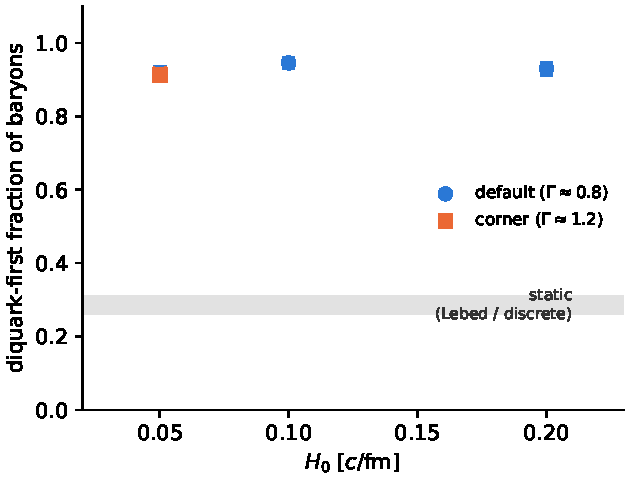
\includegraphics[width=\columnwidth]{figs/fig9_dqfirst.pdf}
\caption{Diquark-first fraction of baryons versus expansion rate at two
couplings, compared with the static nearest-neighbor band evaluated at
the simulation density ($n_0R^3=1$; band spans the Lebed and
discrete-color countings).  Dynamics amplifies the static probability
toward unity.}
\label{fig:dqfirst}
\end{figure}
